%*******10********20********30********40********50********60********70********80

\chap{Background Theory} 

The background theory required for implement this thesis work could be basically divided into 4 main areas:
\begin{itemize}
\item Data science
\item Aquaculture in Norway
\item Machine Learning
\item Python
\end{itemize}

Could be very useful to give some basic definitions and explanations about the topics written just above and then try to get some more specific informations during the course of this thesis.

\newpage
\section{Data science}
We can define Data Science like a "concept to unify statistics, data analysis and their related methods" in order to "understand and analyze actual phenomena" with data.
It includes theories drawn from many field within the broad areas of mathematics, statistics, information science and computer science.

In the computer science area in particular the subdomains of machine learning, classification, cluster analysis, data mining, databases, and visualization.
The follow image represents the "Blitzstein and Pfister's framework" and provides a clear overview of the topic.

\begin{figure}[h]
    \centering
    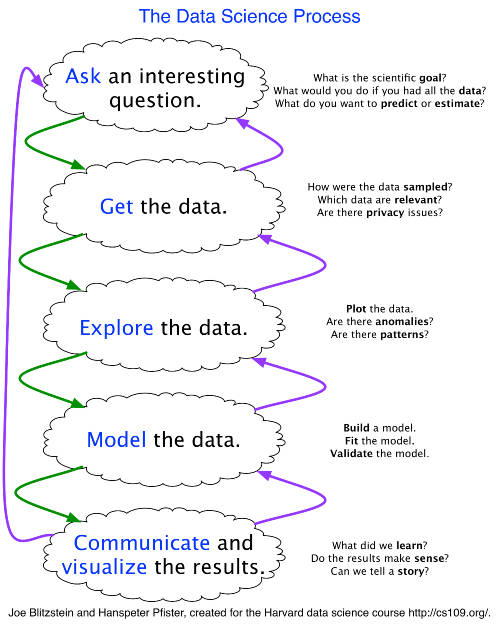
\includegraphics[trim=0cm 0.7cm 0cm 0cm, clip=true, width=0.8\textwidth,natwidth=610,natheight=642]{Files/Data_Science_Process_2.jpg}
    \caption[Data science process]{Data science process}
    \label{fig: Data_science}
\end{figure}

\section{Aquaculture in Norway}
Aquaculture, also known as aquafarming, is the farming of fish, crustaceans, molluscs, aquatic plants, algae, and other aquatic organisms.

Aquaculture would be the future of fish:
In 2030, according to the World Bank, aquaculture will supply:
\begin{itemize}
\item 93.6 Million tonnes of fish per year
\item 25 percent less wild fish will be available
\item 62 percent of the fish we eat will come from farms
\end{itemize}


\section{Machine learning}
This subfield of computer science gives "computers the ability to learn without being explicitly programmed". \\Evolved from the study of pattern recognition and computational learning theory in artificial intelligence,[2] machine learning explores the study and construction of algorithms that can learn from and make predictions on data.

There are several machine learning algorithm, each one of them is used for a different purpose.The following picture gives a general idea about which categories of algorithms are used and some specific types.
\begin{figure}[h]
    \centering
    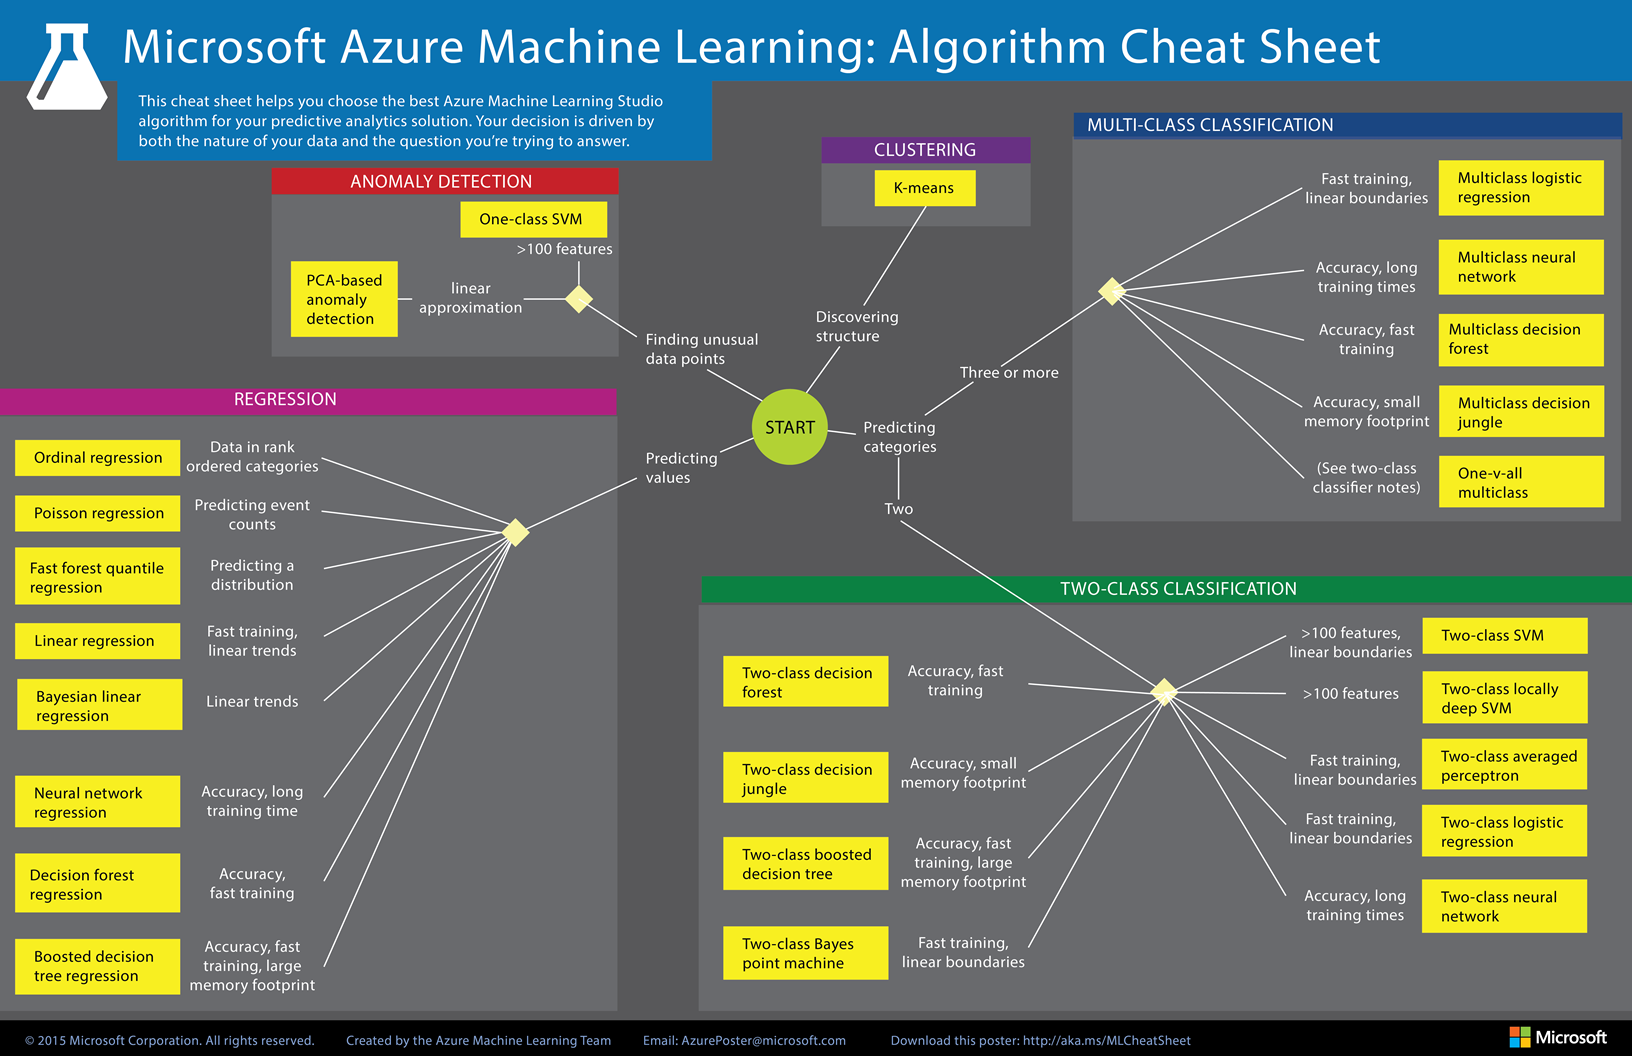
\includegraphics[trim=0cm 0cm 0cm 0cm, clip=true, width=0.8\textwidth,natwidth=610,natheight=642]{Files/Machine_Learning.png}
    \caption[Machine learning algorithms]{Machine learning algorithms}
    \label{fig: Machine_Learning}
\end{figure}



\section{Python}


